\section{Results}

\subsection{Summary of Data and Model Selection}

Analysis of 1,894 paired observations from 115 monitoring periods at two overwintering sites during the 2023-2024 season revealed that environmental factors, but not wind, drove monarch abundance changes. Testing of 47 candidate models identified M23 as the best-fit model.

Model M23 included smooth terms for previous butterfly count, average temperature, butterflies in direct sunlight, and minutes since sunrise, achieving an AIC value of 8081.848 (Table \ref{tab:model_selection}). This model carried 88\% of the support among all candidate models (AIC weight = 0.88), with the next-best model (M22) showing substantially less support (ΔAIC = 4.796). Notably, model M24, which included maximum wind gust as an additional predictor, performed worse than M23 (ΔAIC = 6.2), and wind variables appeared in none of the top-performing models.

\begin{table}[htbp]
\centering
\caption{Model selection results showing the top five candidate models ranked by AIC. Model terms are shown with their respective AIC values, ΔAIC relative to the best model, and AIC weights. Wind p-values are shown where applicable; NA indicates the model did not include wind variables.}
\label{tab:model_selection}
\begin{tabular}{lllrrr}
\hline
Model & Terms & AIC & ΔAIC & Weight & Wind p \\
\hline
M23 & Lagged butterflies, Temperature, & 8081.8 & 0.0 & 0.880 & NA \\
    & Sun exposure, Time of day & & & & \\
M22 & Lagged butterflies, Temperature (linear), & 8086.6 & 4.8 & 0.080 & NA \\
    & Sun exposure, Time of day & & & & \\
M24 & Lagged butterflies, Max gust, Temperature, & 8088.0 & 6.2 & 0.040 & 0.218 \\
    & Sun exposure, Time of day & & & & \\
M47 & Temperature, Sun exposure, & 8101.3 & 19.4 & <0.001 & NA \\
    & Time of day & & & & \\
M17 & Lagged butterflies, Temperature, & 8105.9 & 24.0 & <0.001 & NA \\
    & Sun exposure & & & & \\
\hline
\end{tabular}
\end{table}

\subsection{Analysis of the Best-Fit Model}

The best-fit model (M23) explained a modest but significant portion of variance in monarch abundance changes (adjusted R² = 0.057). The model formula was:

\begin{equation}
\text{Change in abundance} \sim s(\text{Previous count}) + s(\text{Temperature}) + s(\text{Sun exposure}) + s(\text{Minutes since sunrise})
\end{equation}

where $s()$ denotes smooth terms. All four smooth terms showed significant effects on monarch abundance changes (Table \ref{tab:smooth_terms}).

\begin{table}[htbp]
\centering
\caption{Summary of smooth terms in the best-fit model (M23). EDF represents effective degrees of freedom, indicating the complexity of each smooth relationship.}
\label{tab:smooth_terms}
\begin{tabular}{lrrrr}
\hline
Term & EDF & Ref. df & F-value & p-value \\
\hline
Lagged roost size & 2.62 & 2.62 & 12.02 & 8.26e-07 \\
Average temperature & 3.93 & 3.93 & 3.23 & 0.028 \\
Direct sun exposure & 1.53 & 1.53 & 19.36 & 1.22e-05 \\
Time within day & 4.90 & 4.90 & 8.90 & <2e-16 \\
\hline
\end{tabular}
\end{table}

The previous butterfly count showed a significant non-linear negative relationship with abundance change (EDF = 2.62, F = 12.02, p < 0.001). As the initial roost size increased, the change in abundance became increasingly negative, indicating proportionally greater departures from larger aggregations (Figure \ref{fig:effect_roost_size}). Average temperature exhibited a complex non-linear relationship (EDF = 3.93, F = 3.23, p = 0.028), with effects peaking at approximately 20°C (Figure \ref{fig:effect_temperature}).

\begin{figure}[htbp]
\centering
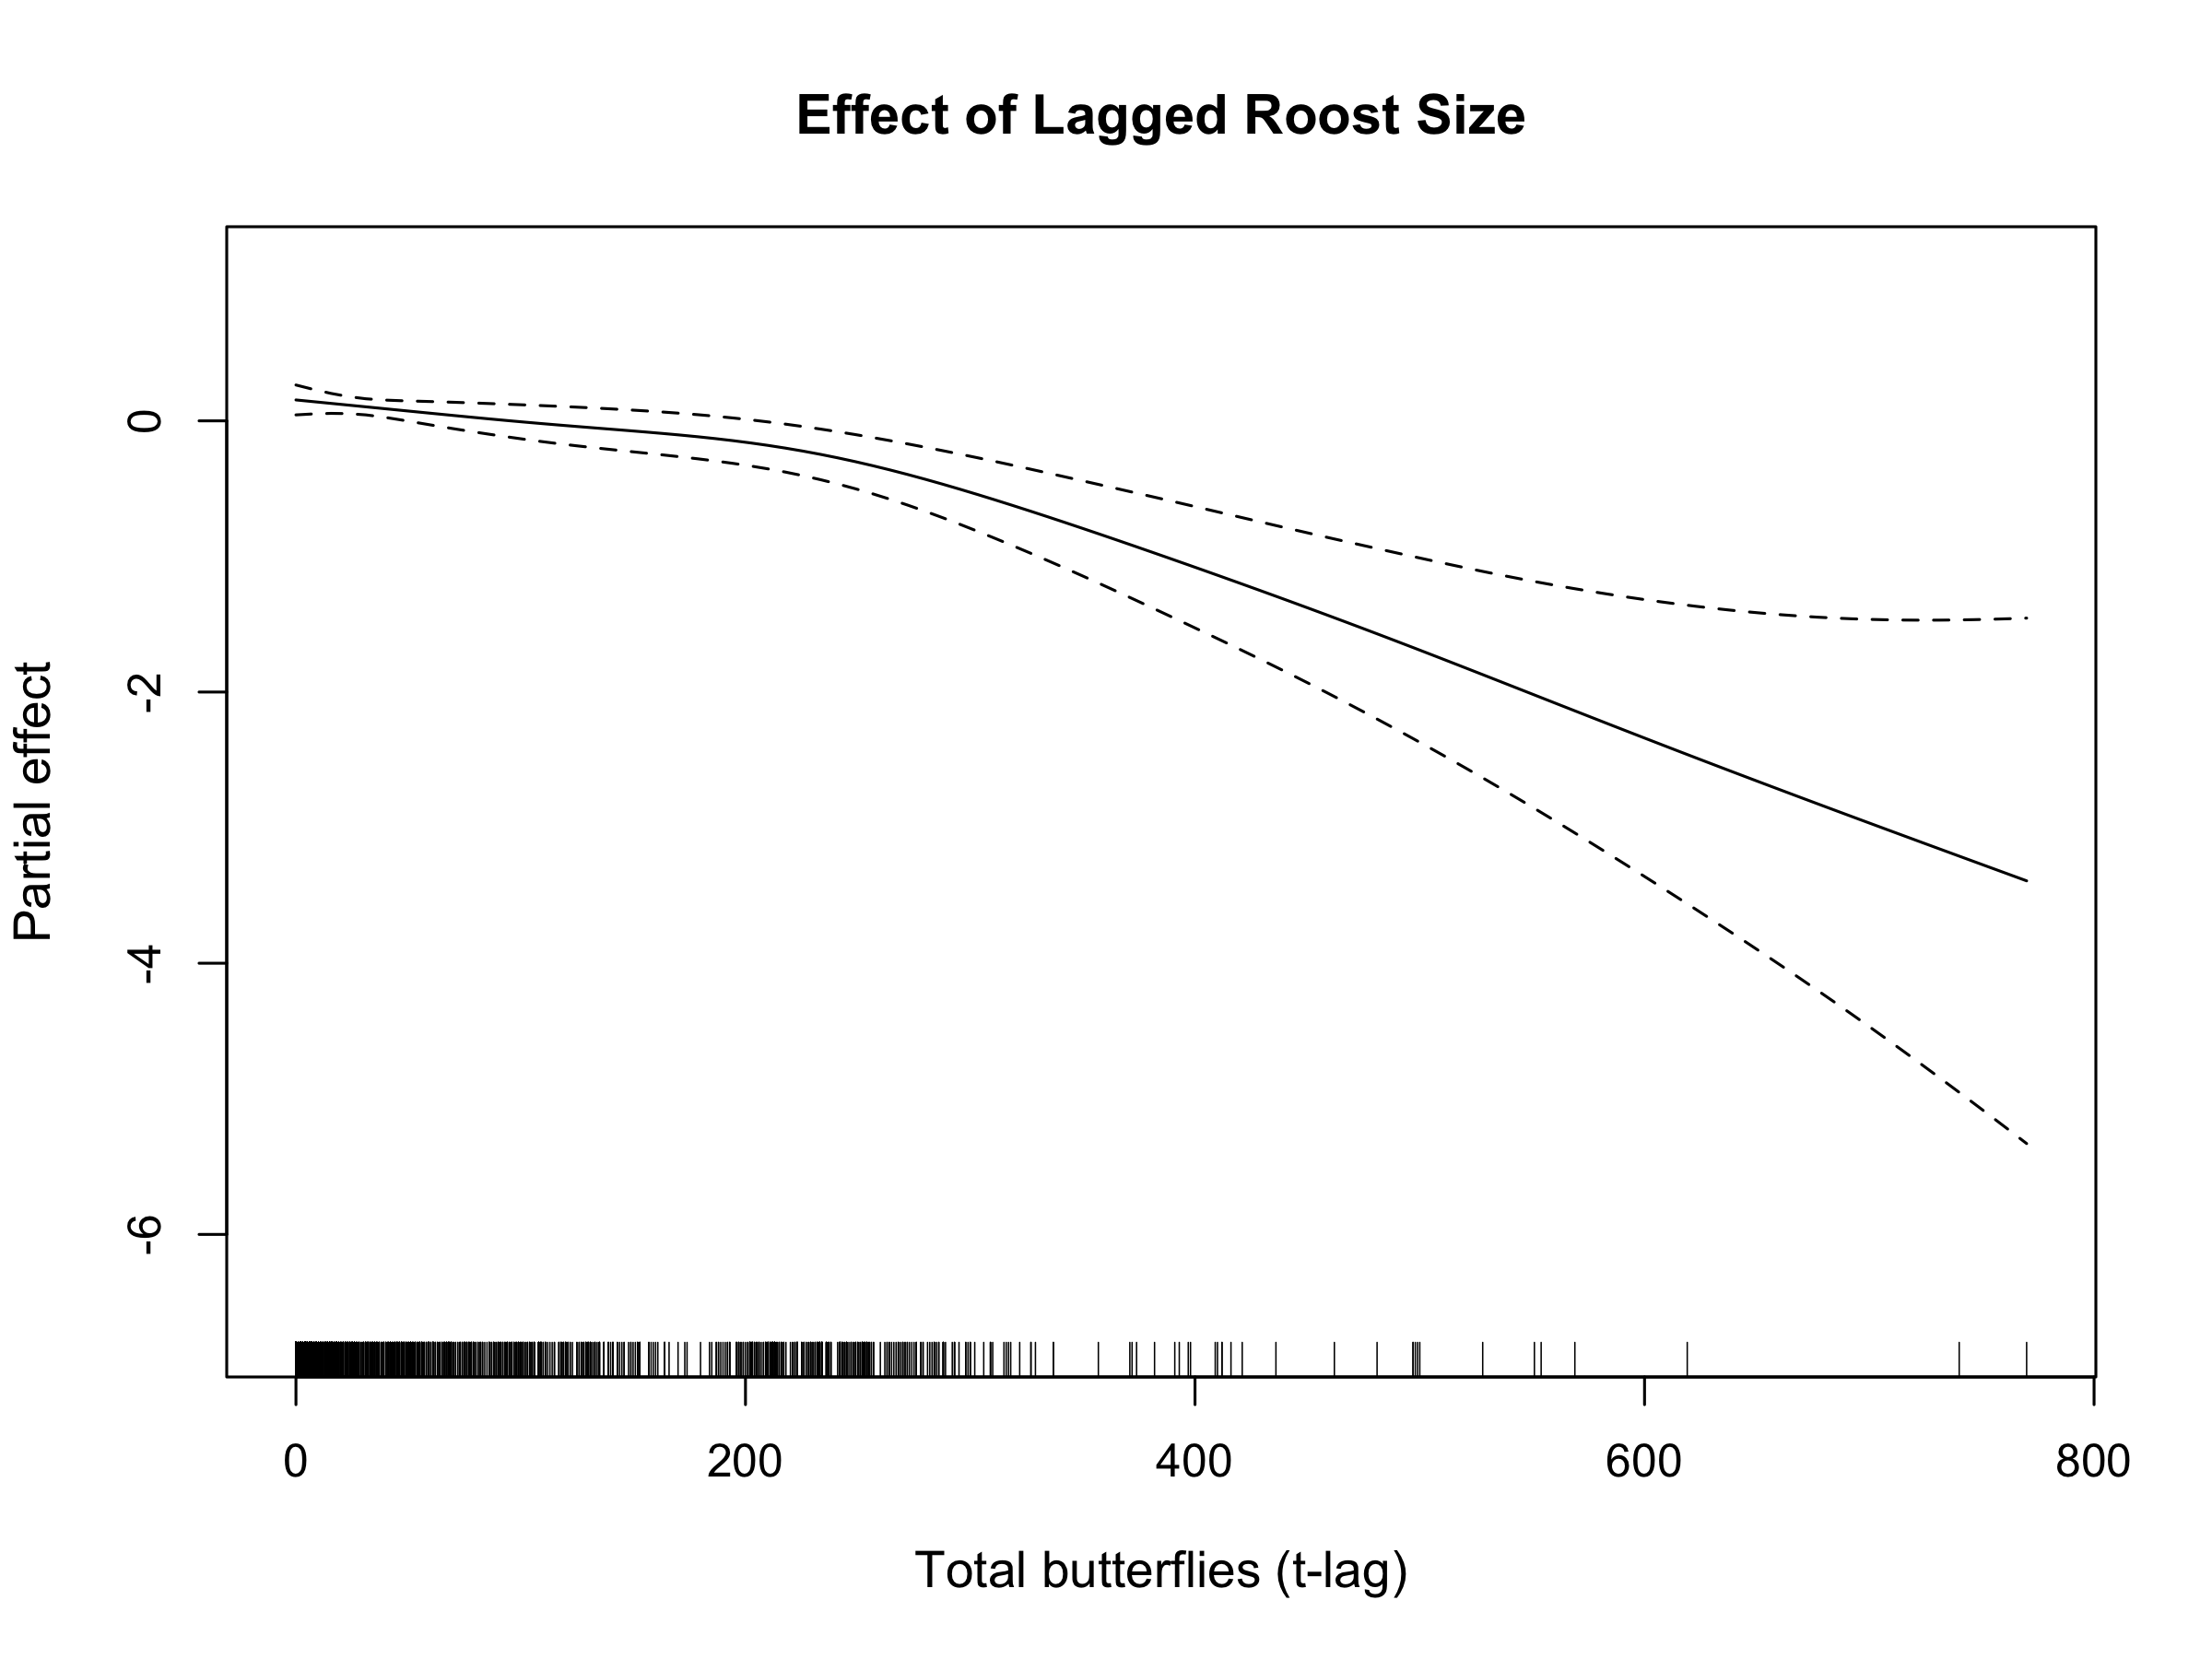
\includegraphics[width=0.8\textwidth]{supplemental/results/thesis_exports/figures/effect_lagged_roost_size.png}
\caption{Partial effect of previous butterfly count on abundance change, showing greater departures from larger roosts. Shaded area: 95\% confidence interval.}
\label{fig:effect_roost_size}
\end{figure}

\begin{figure}[htbp]
\centering
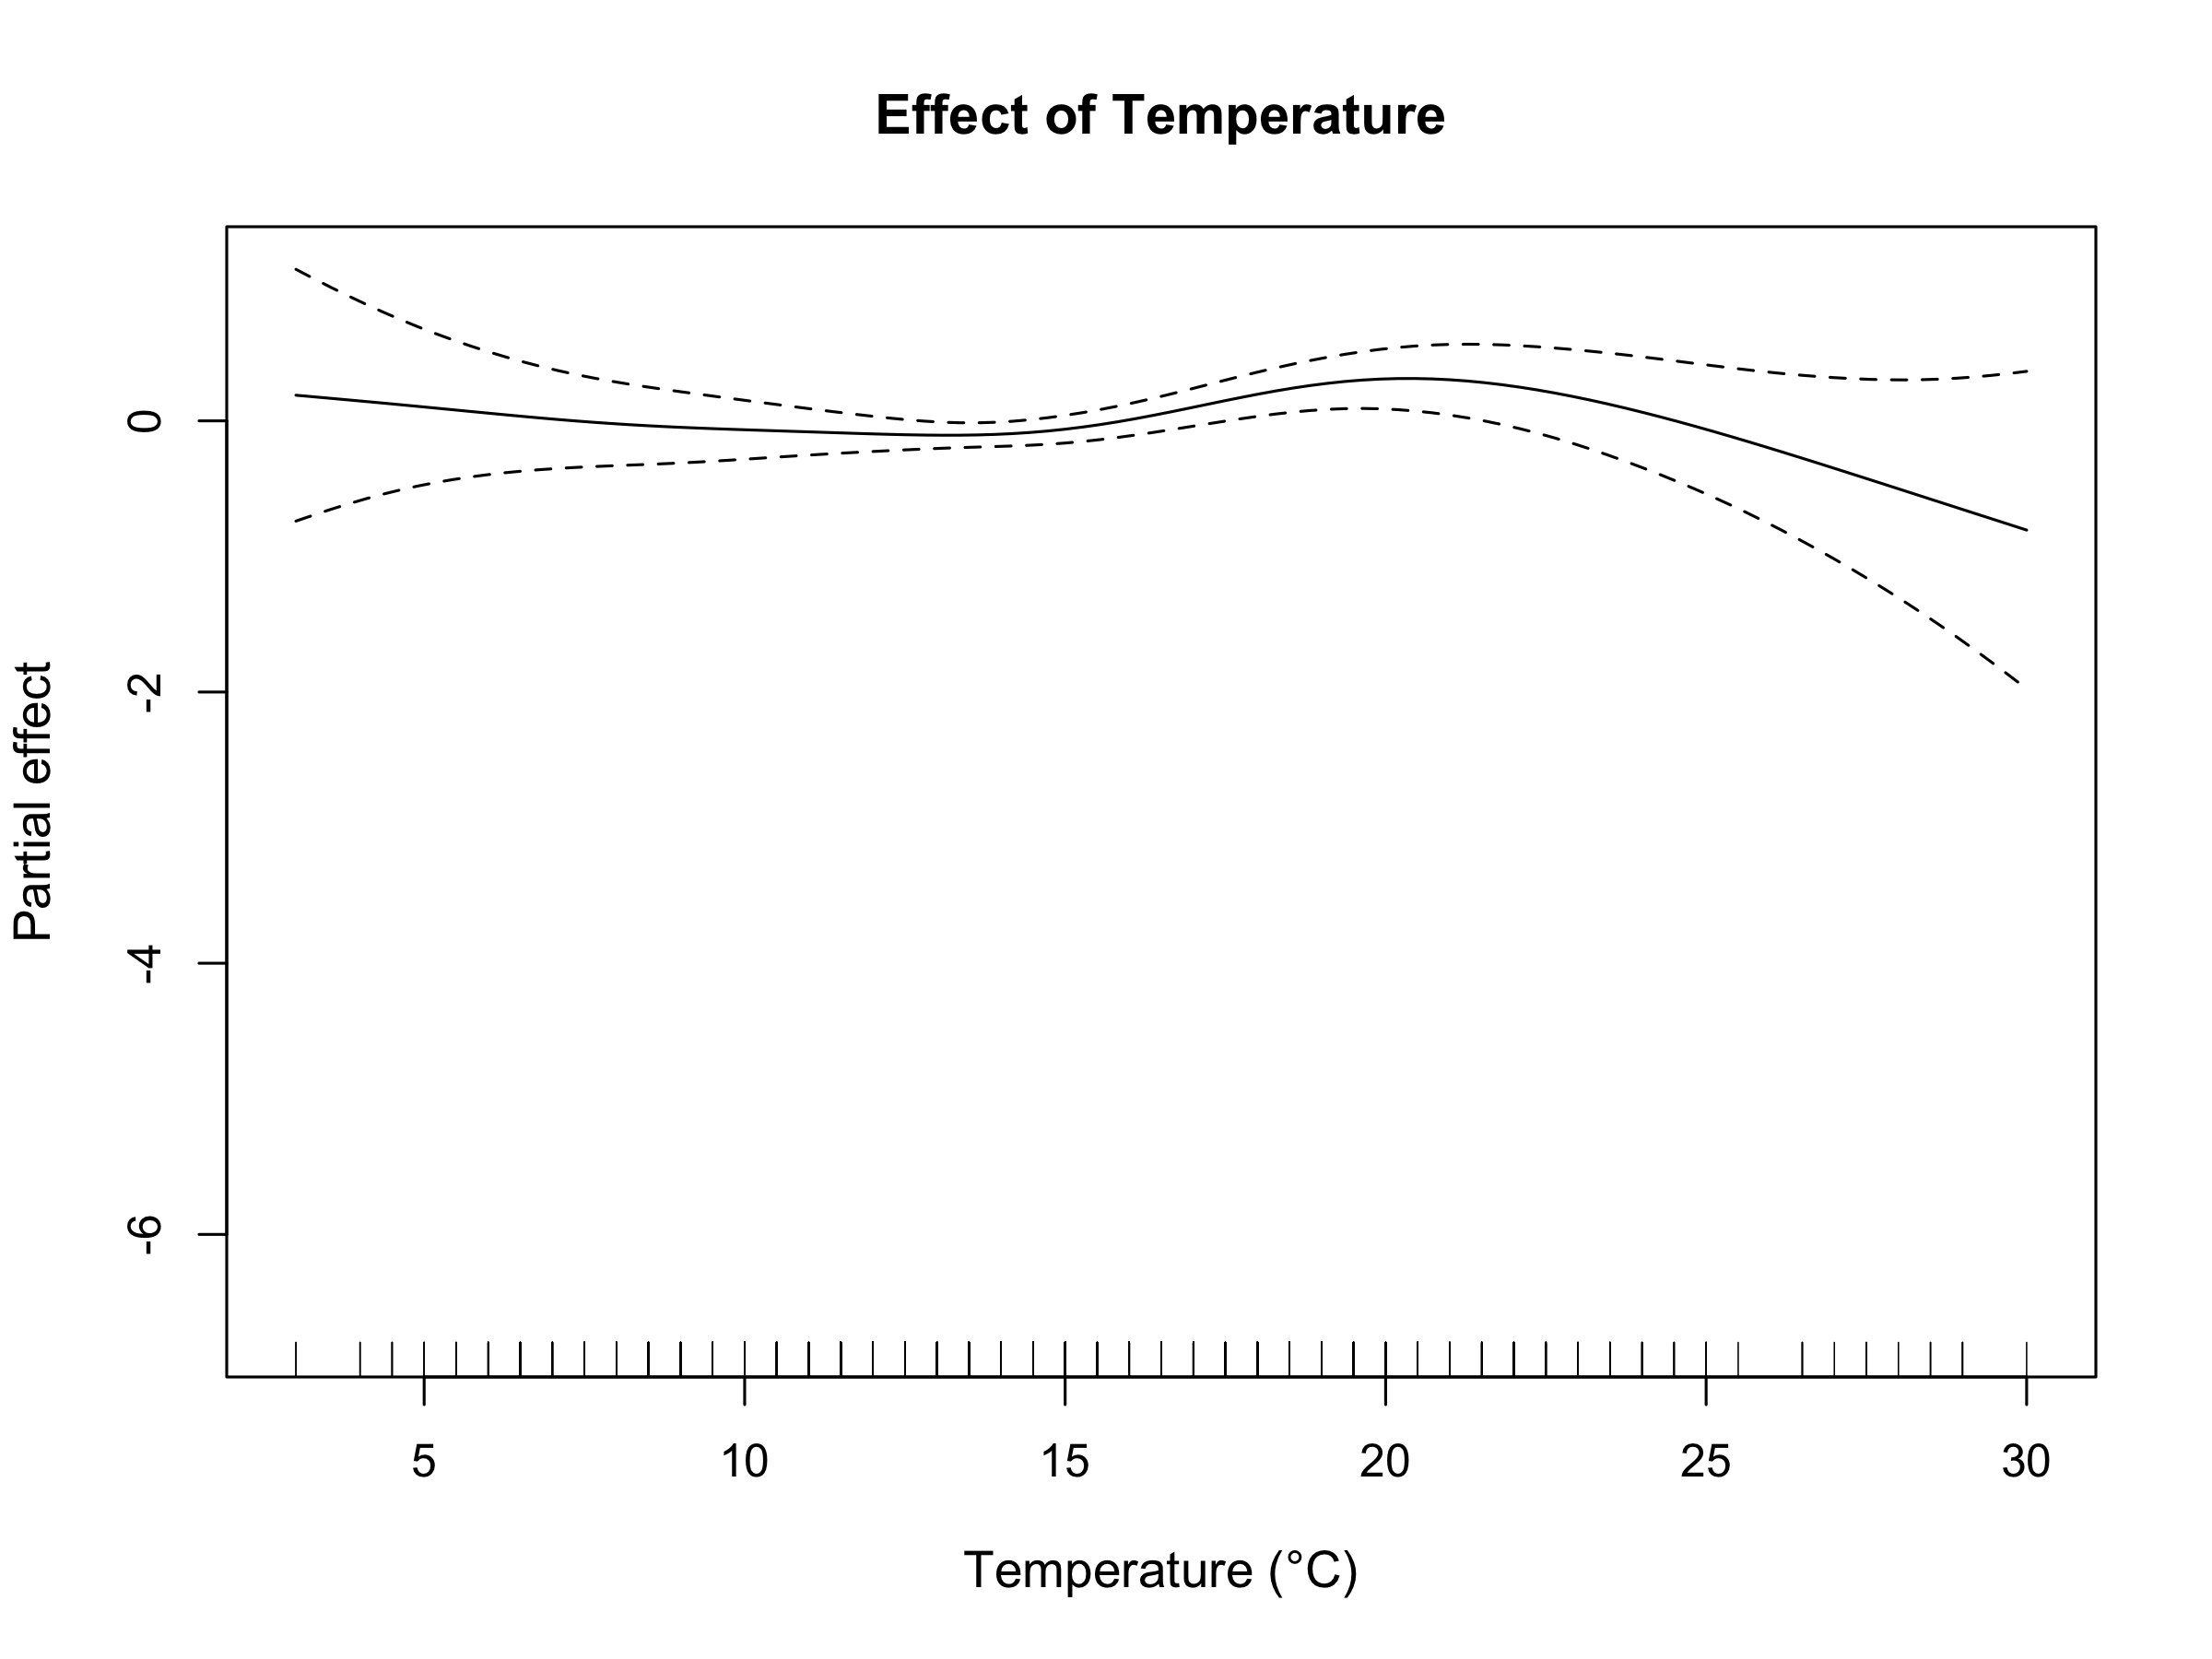
\includegraphics[width=0.8\textwidth]{supplemental/results/thesis_exports/figures/effect_temperature.png}
\caption{Partial effect of temperature on monarch abundance change, peaking at approximately 20°C. Shaded area: 95\% confidence interval.}
\label{fig:effect_temperature}
\end{figure}

Butterflies exposed to direct sunlight showed a strong negative effect on roost abundance (EDF = 1.53, F = 19.36, p < 0.001), with greater sun exposure associated with larger decreases in total abundance (Figure \ref{fig:effect_sun}). This nearly linear relationship suggests a consistent departure response to solar radiation. Minutes since sunrise revealed a pronounced diurnal pattern (EDF = 4.90, F = 8.90, p < 0.001), capturing cyclical changes in monarch activity throughout daylight hours (Figure \ref{fig:effect_diurnal}).

\begin{figure}[htbp]
\centering
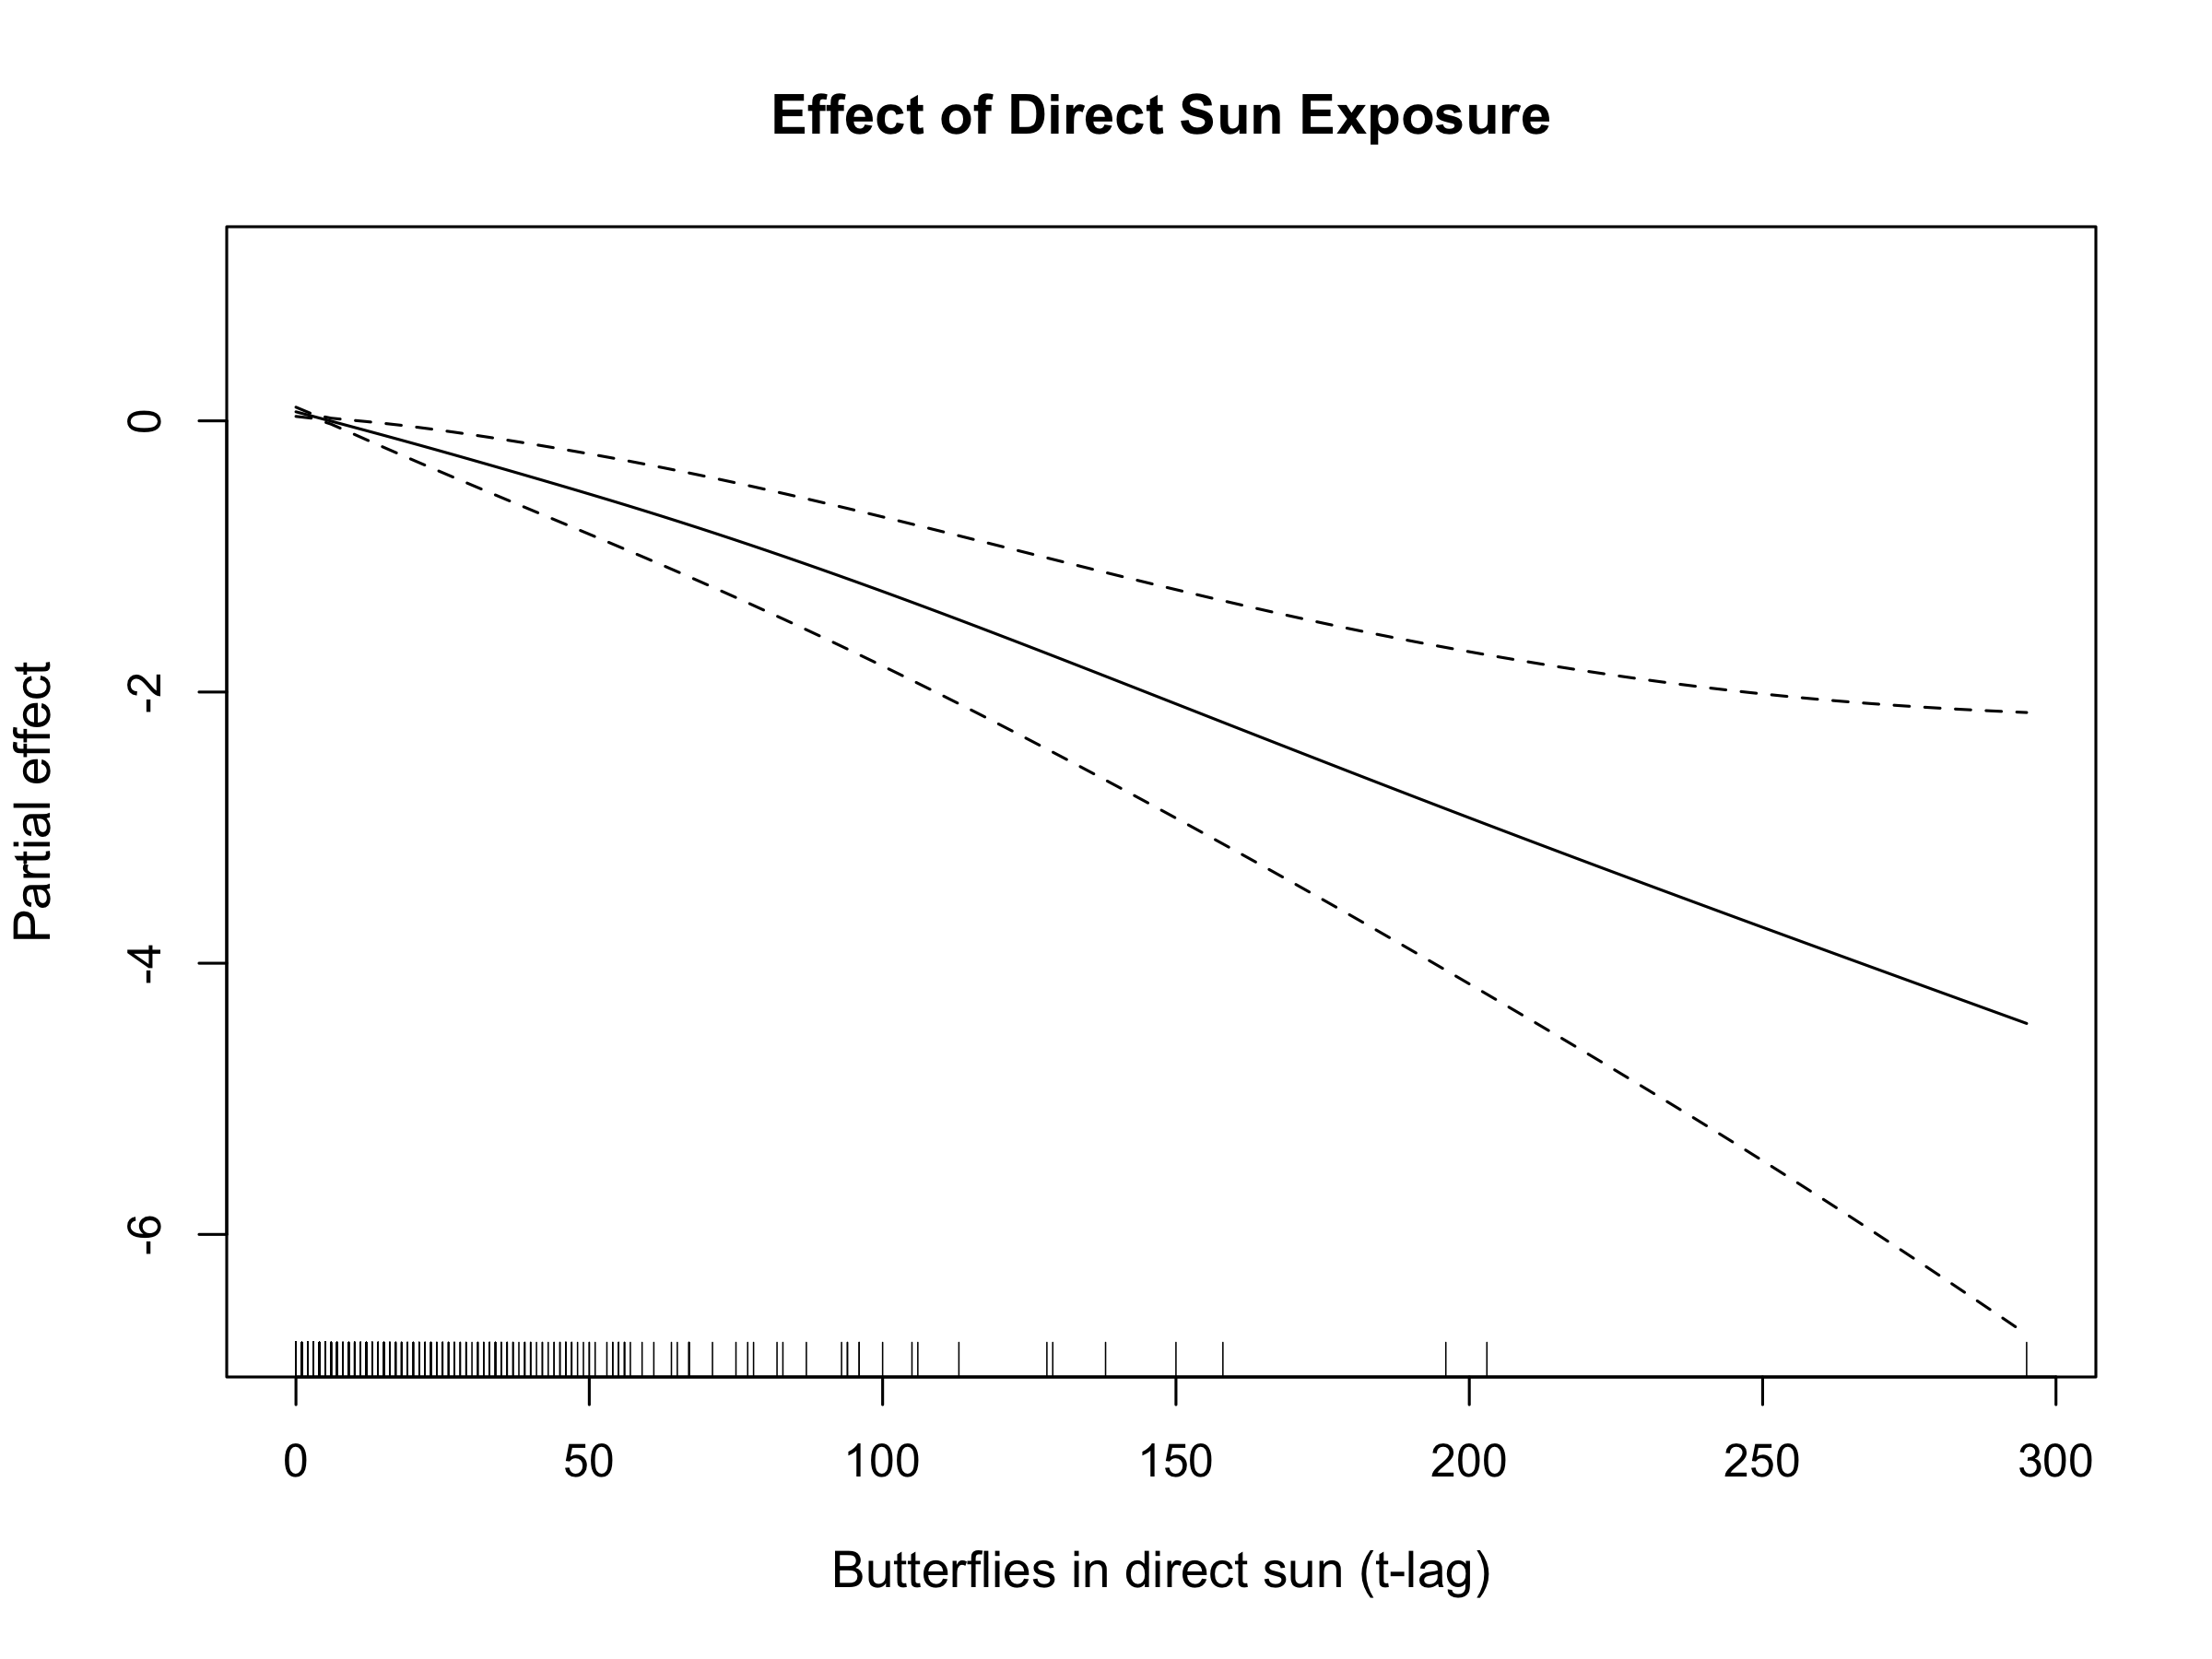
\includegraphics[width=0.8\textwidth]{supplemental/results/thesis_exports/figures/effect_sun_exposure.png}
\caption{Partial effect of sun exposure on abundance change. Greater sun exposure drives departures from the roost. Shaded area: 95\% confidence interval.}
\label{fig:effect_sun}
\end{figure}

\begin{figure}[htbp]
\centering
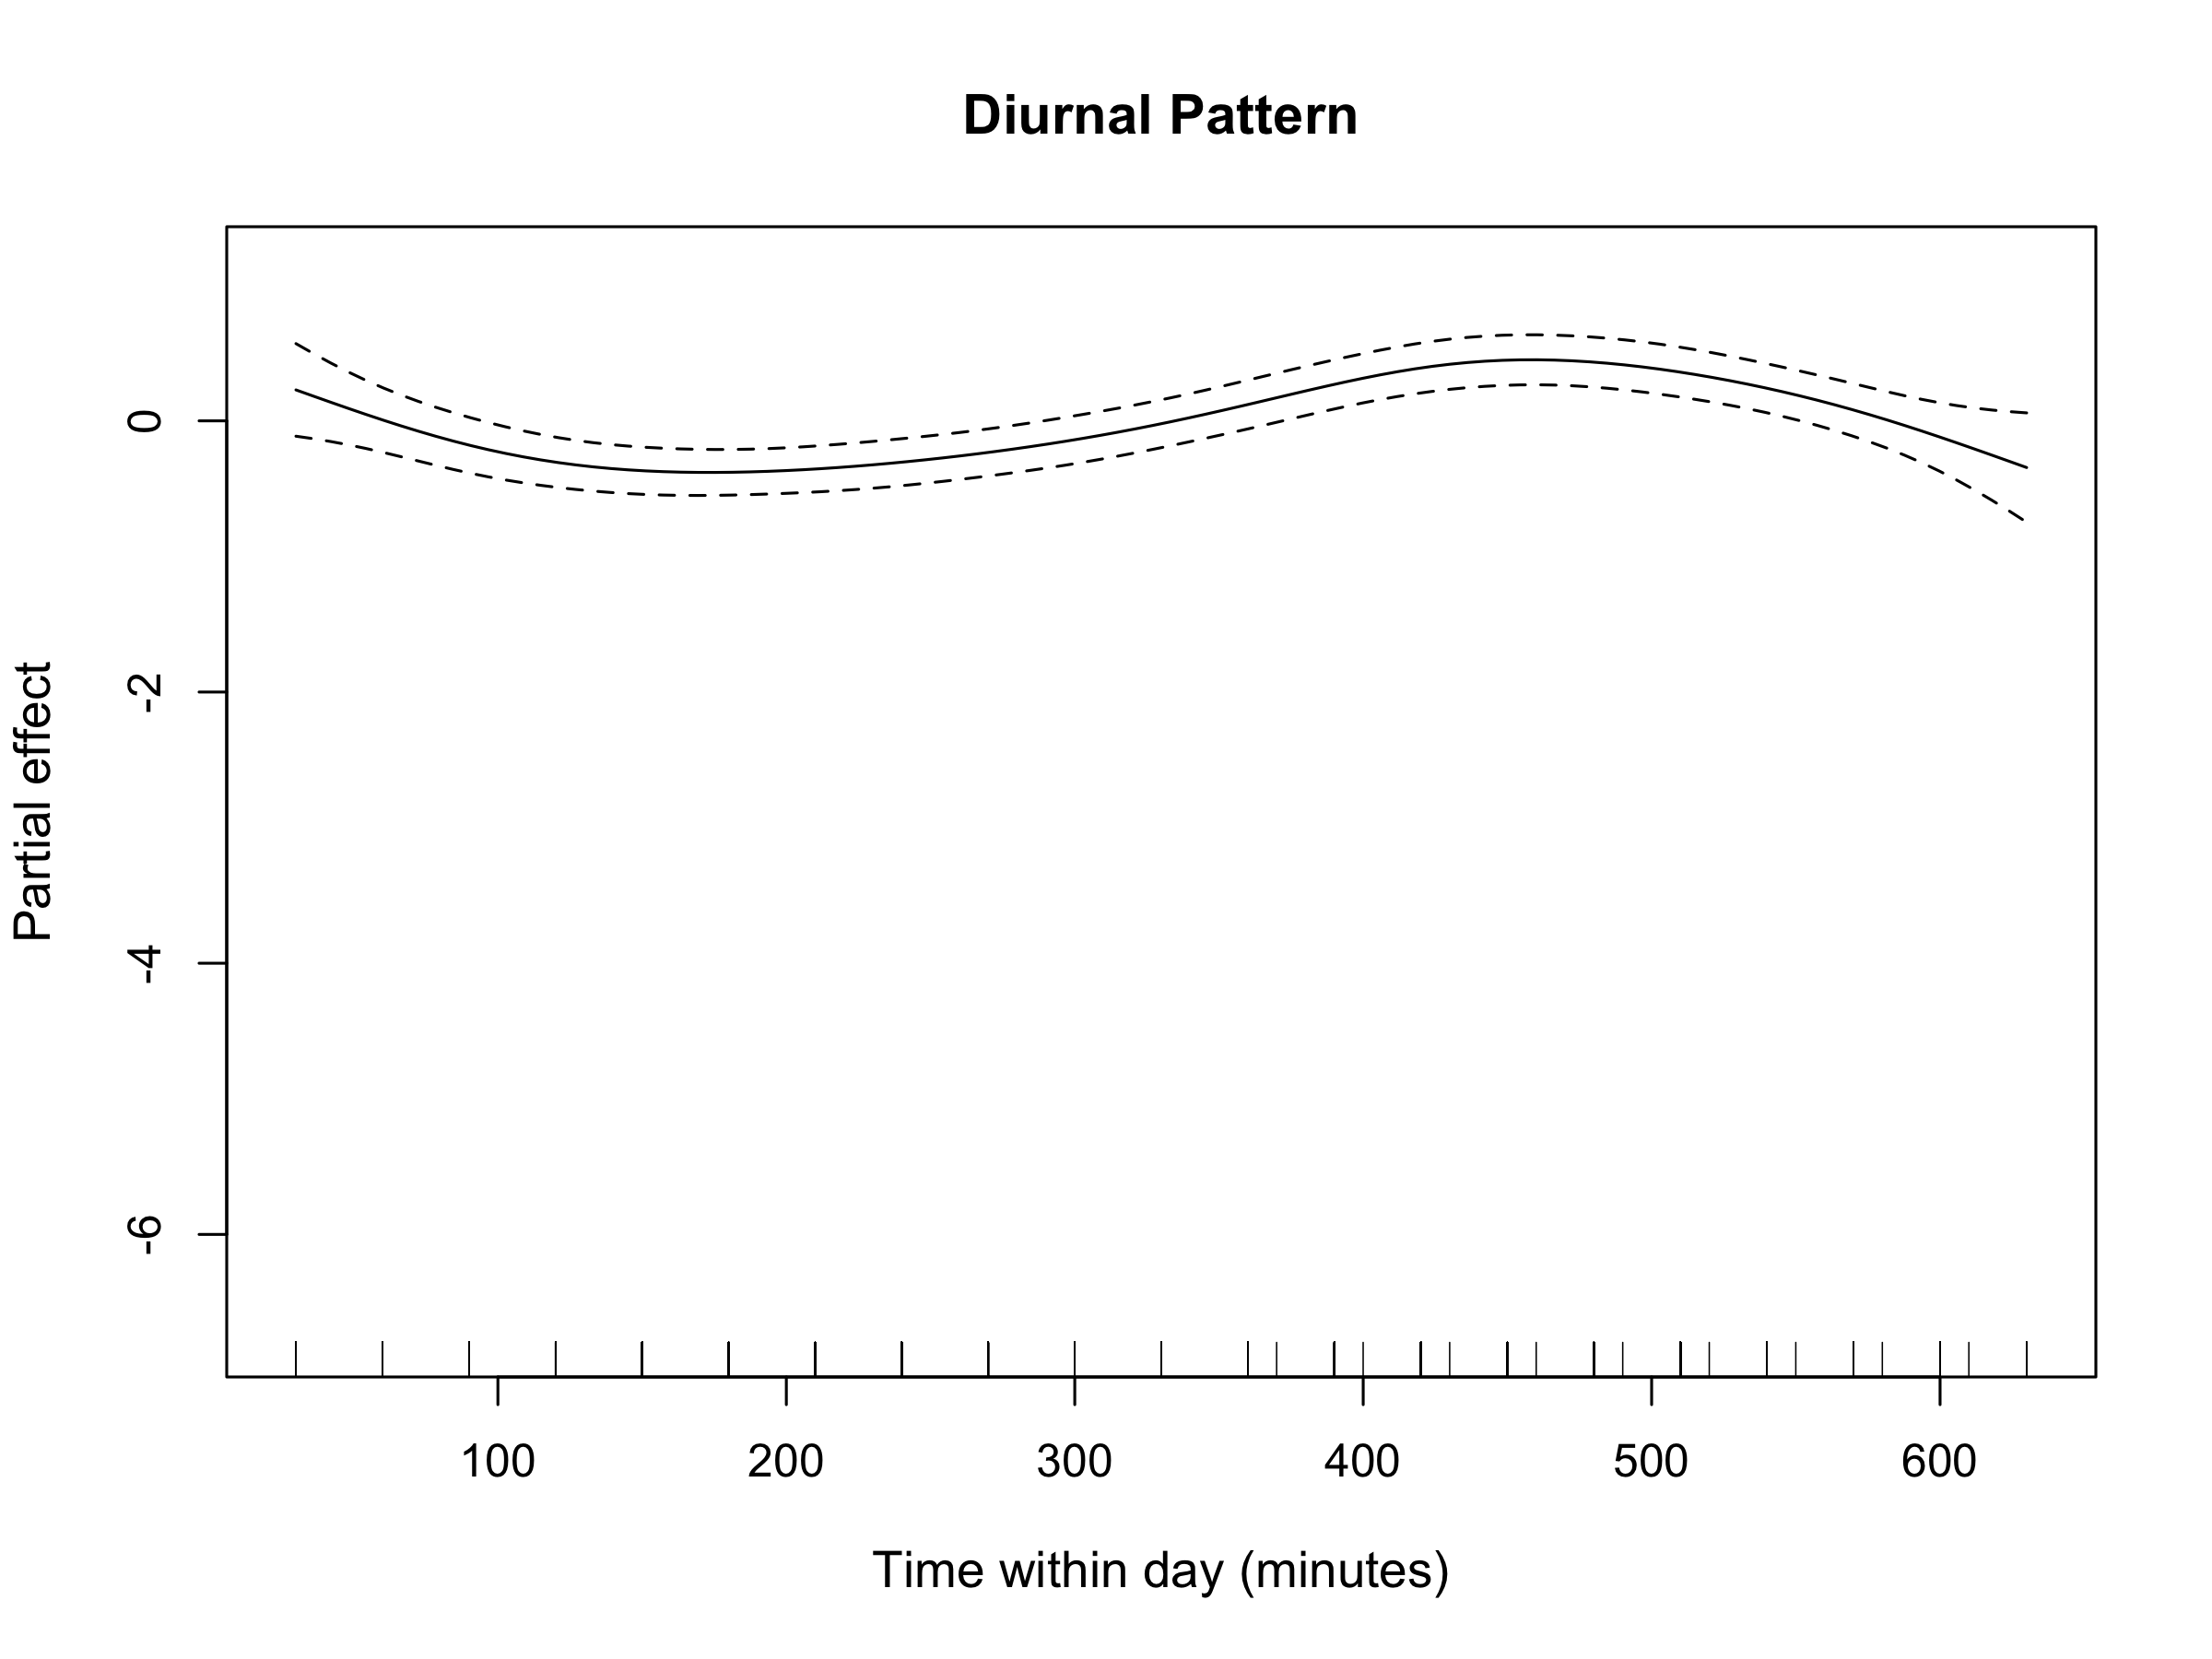
\includegraphics[width=0.8\textwidth]{supplemental/results/thesis_exports/figures/effect_diurnal_pattern.png}
\caption{Diurnal pattern of monarch abundance changes relative to minutes since sunrise. Shaded area: 95\% confidence interval.}
\label{fig:effect_diurnal}
\end{figure}

\subsection{Evaluation of the Disruptive Wind Hypothesis}

Our analysis provided no support for the three hierarchical wind hypotheses:

First, wind did not act as a disruptive force to overwintering monarchs. Wind variables failed to appear in any top-performing models. When maximum gust was forced into the best model structure (M24), model performance declined (ΔAIC = 6.2) and the wind effect was not statistically significant (p = 0.218).

Second, we found no evidence for disruption above the proposed 2 m/s threshold. Despite mean wind gusts averaging 2.2 m/s (SD = 1.4 m/s)—conditions that should have revealed threshold effects if present—no disruption occurred at or above this boundary.

Third, wind's effects did not scale with intensity. Maximum gust speed showed no relationship with monarch abundance changes across the entire observed range (0–8 m/s), with the fitted relationship remaining flat and confidence intervals consistently encompassing zero (Figure \ref{fig:wind_scatter}).

\begin{figure}[htbp]
\centering
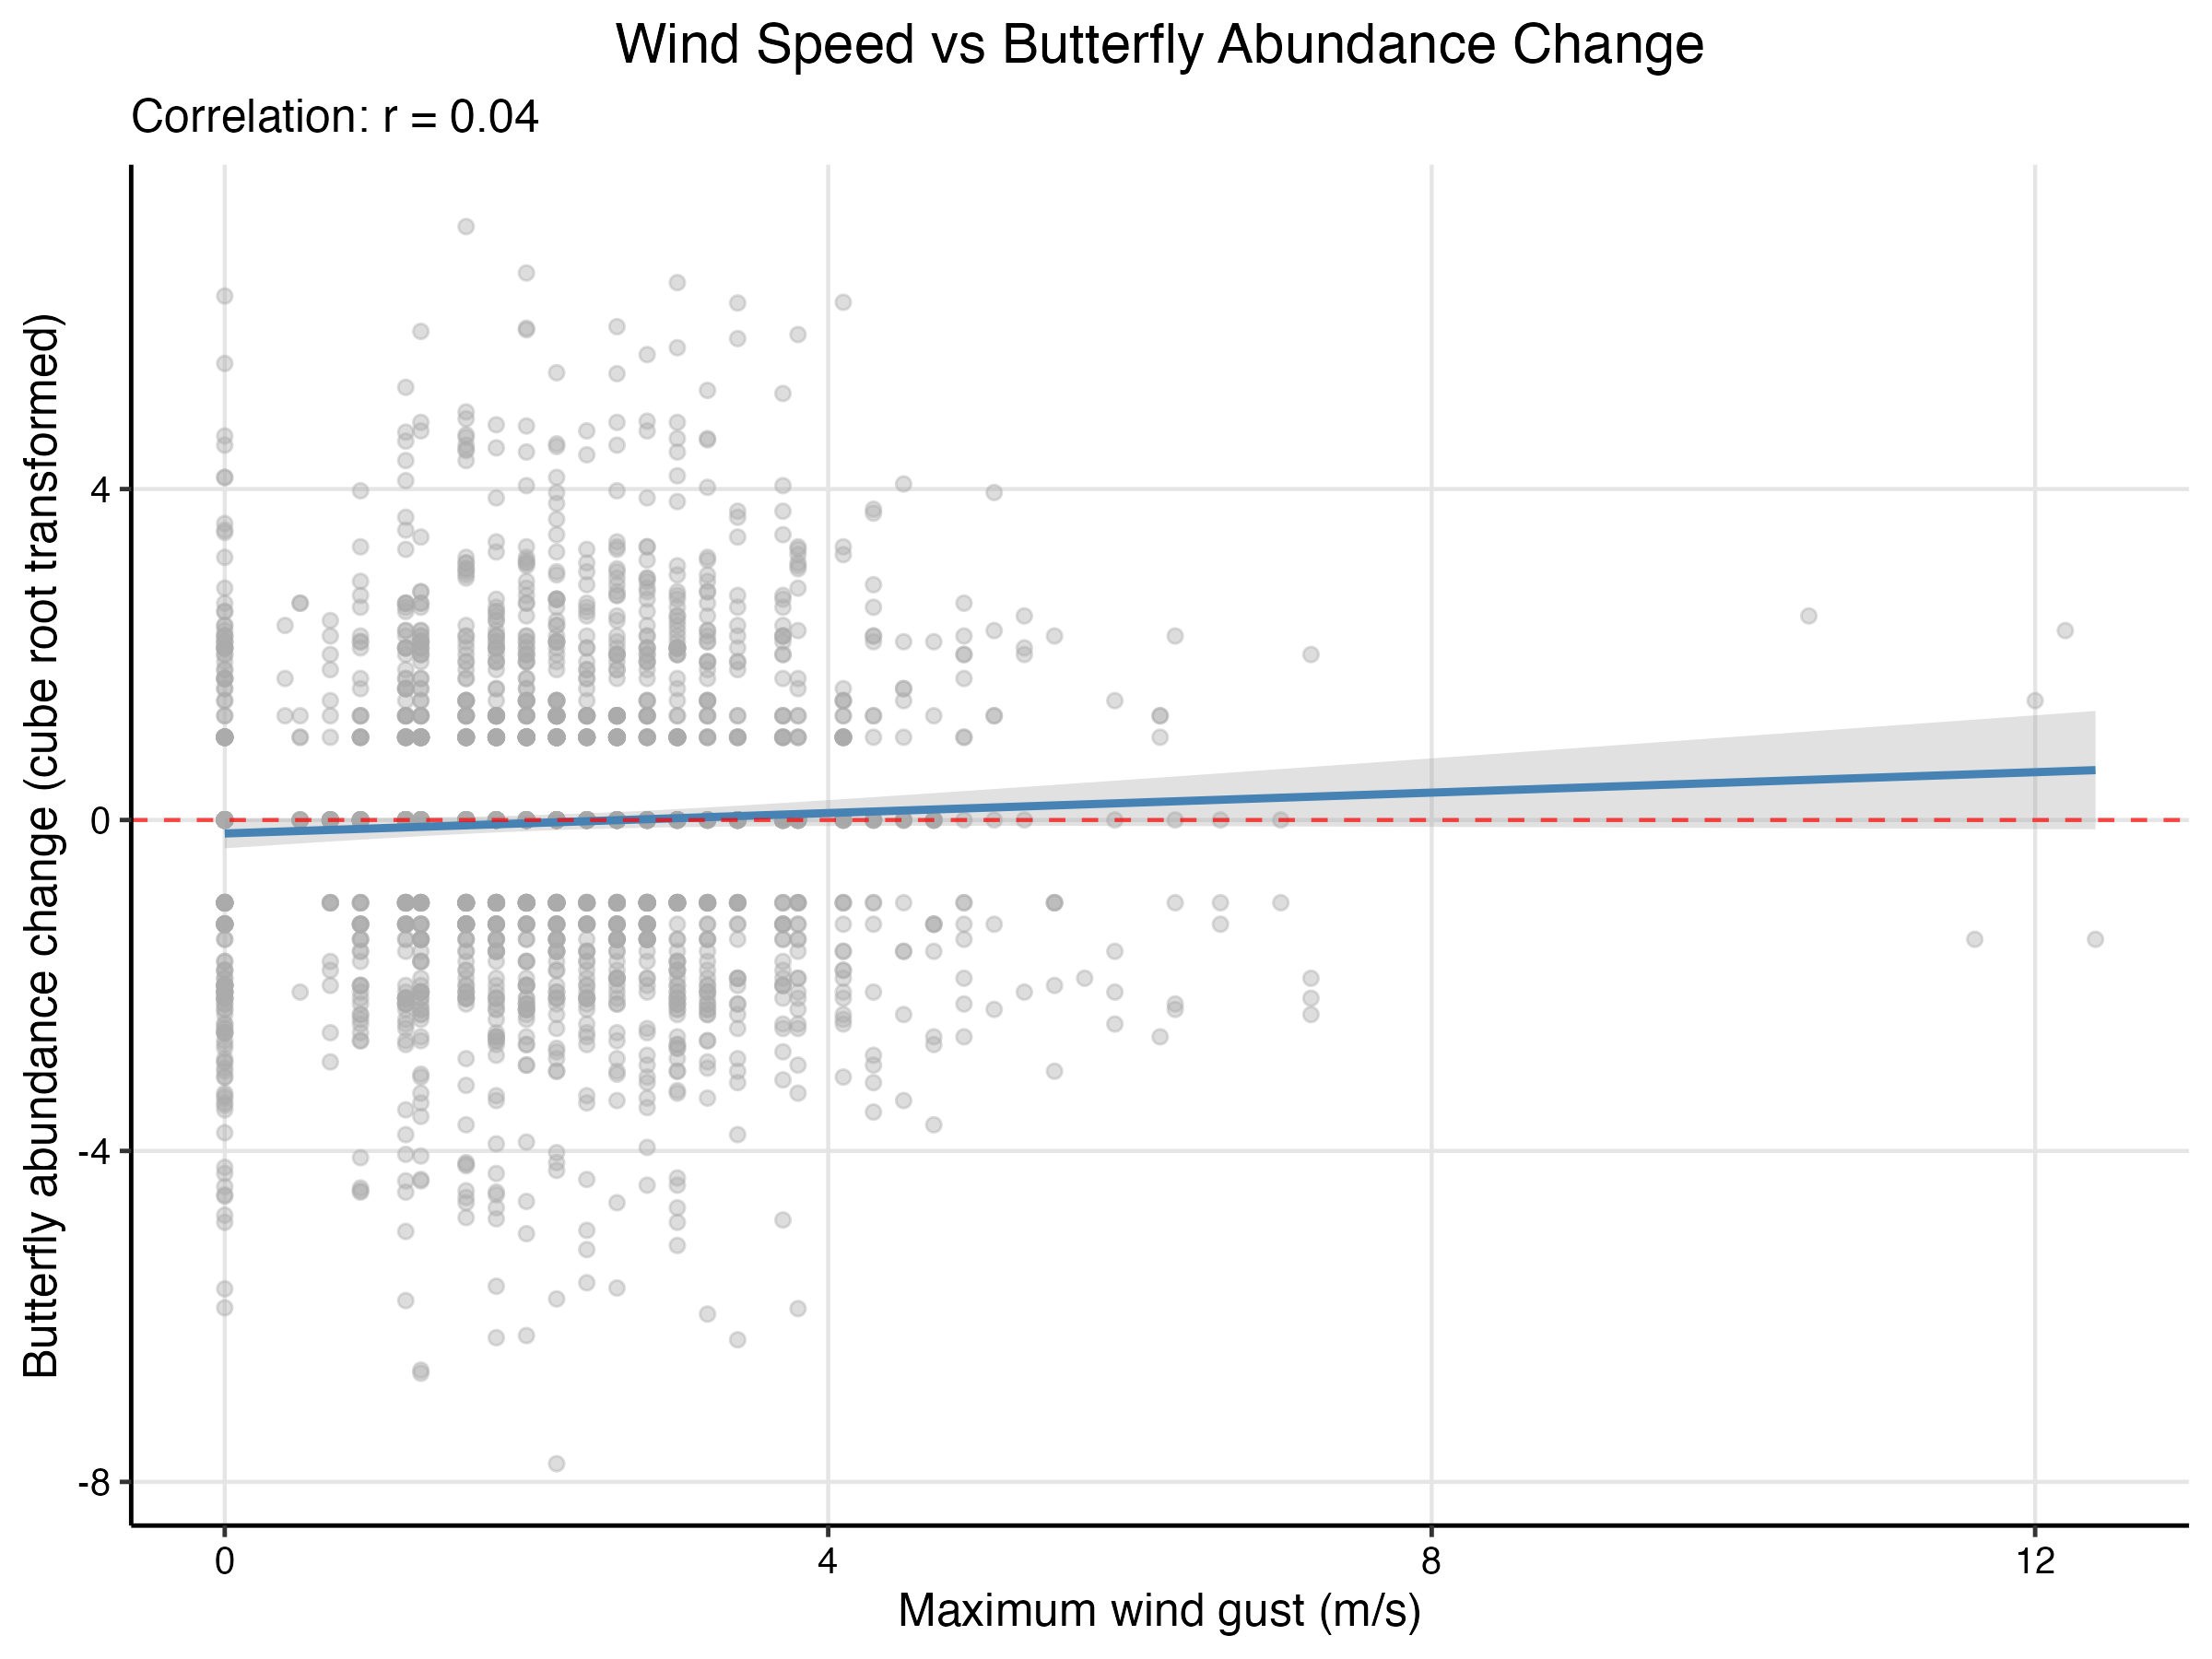
\includegraphics[width=0.8\textwidth]{supplemental/results/thesis_exports/figures/wind_hypothesis_scatter.png}
\caption{Relationship between maximum wind gust speed (m/s) and monarch abundance change. Flat trend line indicates no effect of wind on butterfly departures. Points represent 30-minute observation periods.}
\label{fig:wind_scatter}
\end{figure}

\subsection{Model Diagnostics}

Model residuals showed distinct linear banding patterns consistent with the discrete counting method used to estimate butterfly abundance (Figure \ref{fig:residuals}).

\begin{figure}[htbp]
\centering
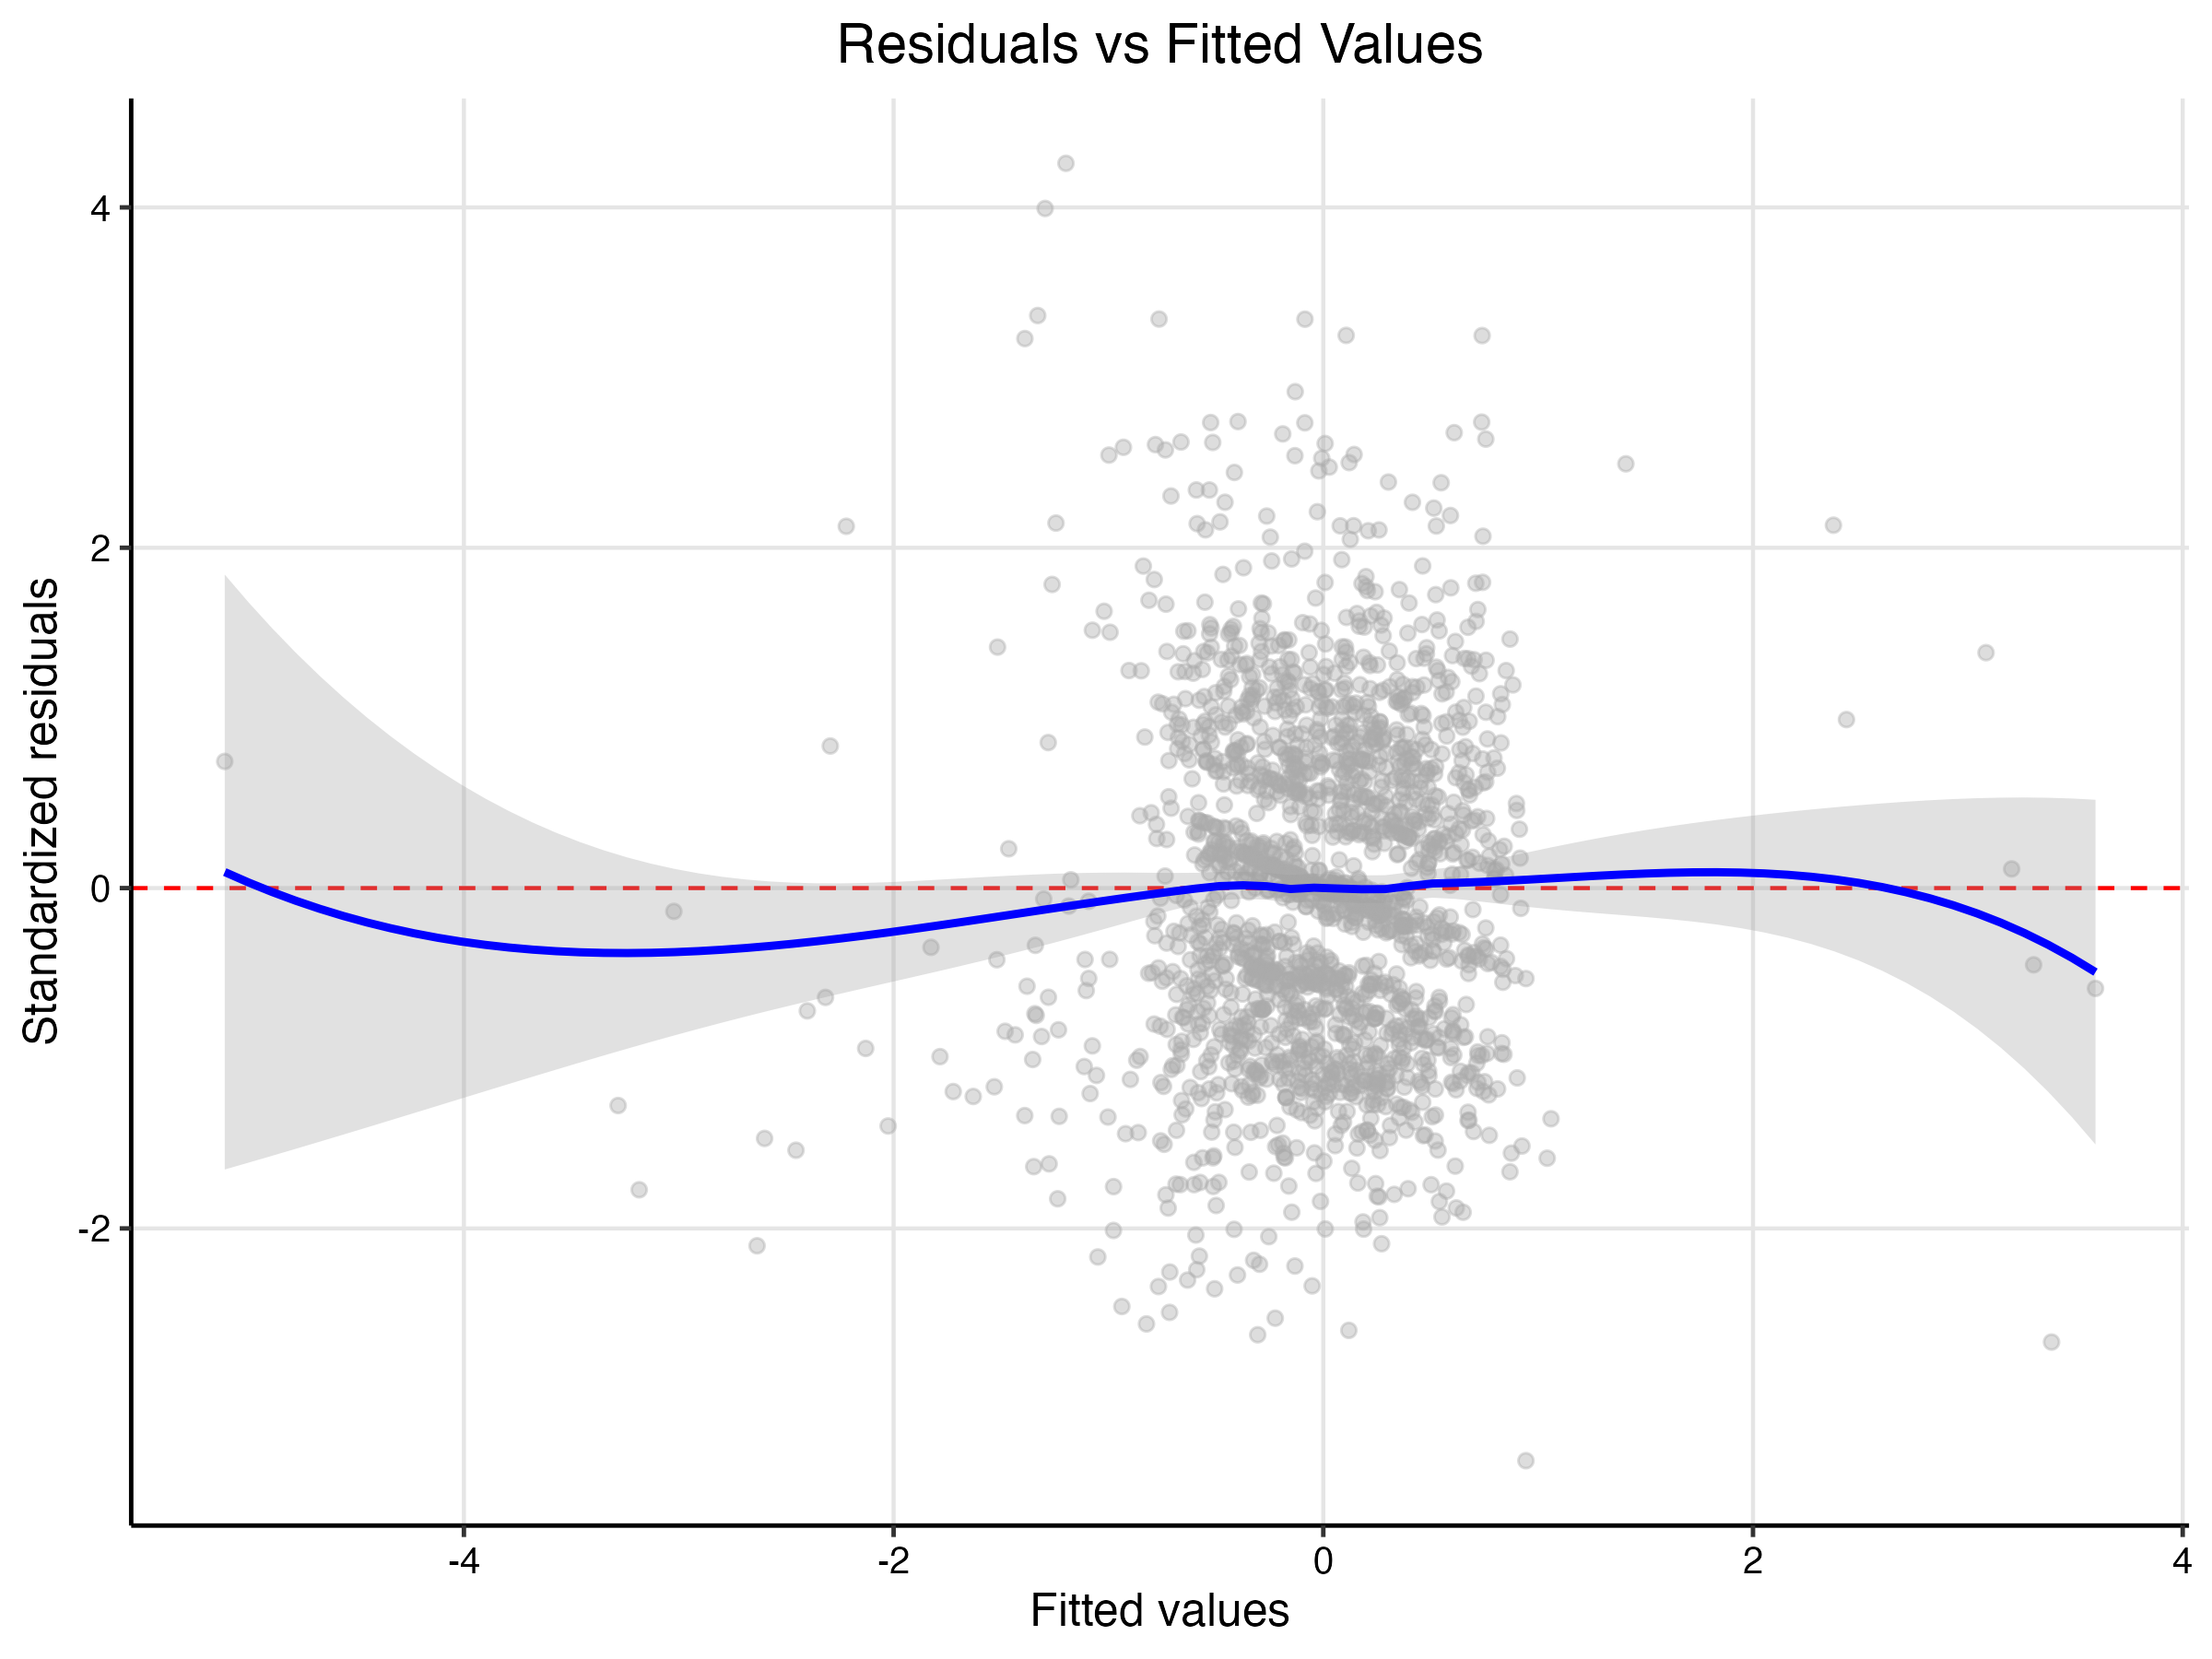
\includegraphics[width=0.8\textwidth]{supplemental/results/thesis_exports/figures/residuals_vs_fitted.png}
\caption{Residuals versus fitted values for model M23. Banding reflects the discrete counting method. Red line: smoothed relationship.}
\label{fig:residuals}
\end{figure}

The Q-Q plot indicated approximately normal residual distribution with minor tail deviations consistent with the discrete counting method (Figure \ref{fig:qqplot}).

\begin{figure}[htbp]
\centering
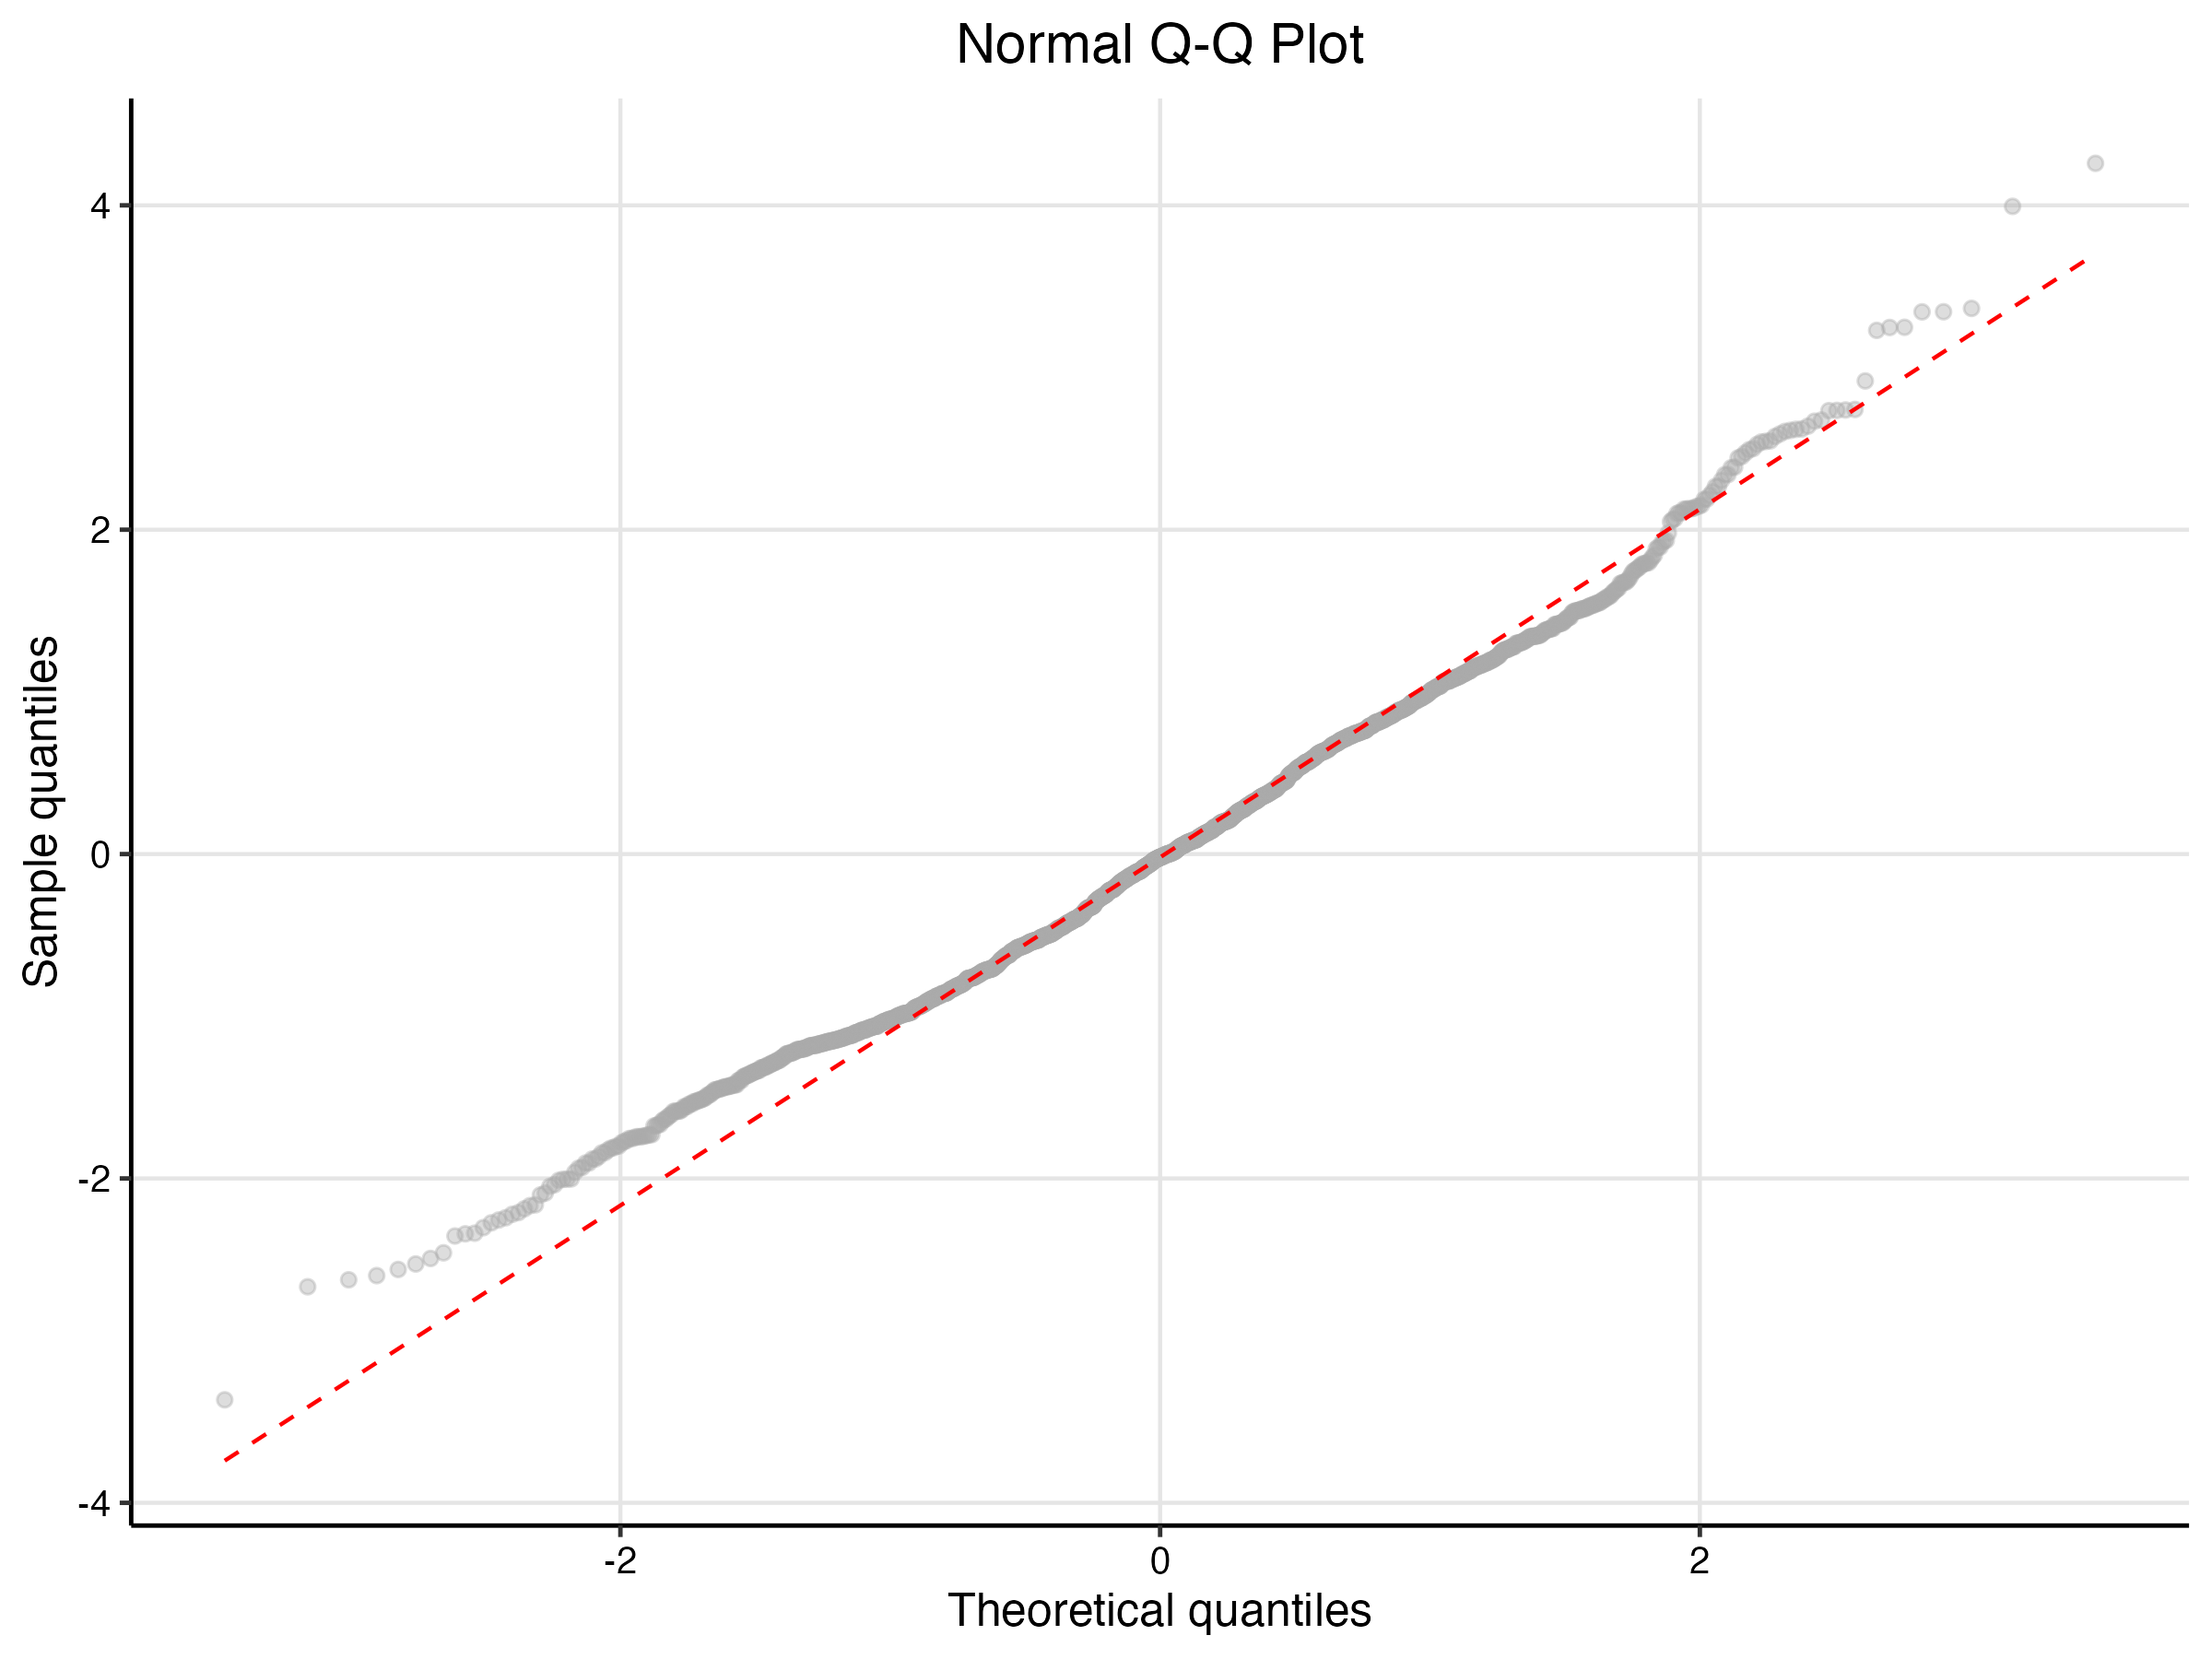
\includegraphics[width=0.8\textwidth]{supplemental/results/thesis_exports/figures/qq_plot.png}
\caption{Q-Q plot of model residuals showing reasonable normality with minor tail deviations from discrete counting.}
\label{fig:qqplot}
\end{figure}
